\section{Python Project Analysis} % {{{

\marginnote{
\includegraphics[width=\marginparwidth]{python/logo}}

Python is an object oriented, interpreted programming language
\cite{PythonAbout}. It is well known for it's simplicity and easy to learn
syntax. Licensed under the \emph{Python Software License} \cite{PythonLicence}
it is widely available for all major platforms. Python comes with an
interpreter and an extensive standard library. It supports many programming
paradigms, such as object oriented, imperative or functional programming
styles. The reference implementation of the interpreter is called
\emph{CPython}, however there are other interpreters available as well. Though
the subject of this analysis will be CPython.

\subsection{History} % {{{

The creator of Python, Guido van Rossum, conceived and implemented Python in
around 1989 at the CWI Institute in the Netherlands \cite{Venners2003}. Python
was a successor to the ABC programming language, which itself saw contributions
from van Rossum in the eighties. The name alludes to the british television
series \emph{Monty Python's Flying Circus} Van Rossum was watching while
creating the programming language. He still is Python's principal author and
project leader and therefore deciding the direction of the project.

Currently, there are two versions of Python available, both incompatible to
each other. Python 2.0 was first released in 2000 and since then evolved to the
currently available Python 2.7 version. Python 3.0 however, was a major,
backwards incompatible release, which was released in 2008. It is the successor
of the 2.x series and will replace it completely in near future.

Also, since the 2.x series, the Python project created a transparent and
community backed development process with van Rossum as it's leader.

\begin{figure}[htbp]
  \centering
  \includegraphics[width=0.8\textwidth]{python/commits_by_author}
  \caption{Monthly activity of the most active Python Core developers. The
  project leader Guido van Rossum appears to be busy with his position as other
  developers such as Georg Brandl are much more active.}
\end{figure}

% }}}

\subsection{Community} % {{{

The Python project has a large user and developer community. Many of these people are
working on the CPython interpreter and the standard library, however there are
also a lot of other Python related projects going on, such as advanced libraries.

The Python community is very eager to attend and offer opportunities to meet in
person. Therefore, one can find a large amount of conferences and workshops
worldwide \cite{PythonConferences}. The first conference was \emph{PyCon} in
North America in 2003. However there are now many other conferences around the
world, such as \emph{PyCon DE}, \emph{EuroPython} and \emph{SciPy}.

The communication inside the Python project is mostly done through several
mailing lists \cite{PythonCommunication}. Each mailing list stands for a
certain topic, for example the \emph{python-dev} mailing list is the main
communication channel for Python development. The python-ideas mailing list on
the other hand is for future ideas and goals of the Python project. There are
of course also other communication methods available, such as several \ac{IRC}
channels and the blogs of the developers.

Next to the already mentioned users and developers of Python people will be
classified into several categories, depending on how much they are involved in
the development of Python \cite{PythonCoreDeveloper}.

\begin{figure}[htbp]
  \centering
  \includegraphics[width=0.8\textwidth]{python/commits_by_year}
  \caption{Yearly overview of commits to CPython. The two peaks appear to match
  the releases of the major releases Python~2 and Python~3.}
\end{figure}

\paragraph{Developer}

One is able to gain the \emph{Developer} role when he has consistently shown
contributions to Python. There is however no set rule of how many patches or
resolved issues are needed. It is possible to request the Developer role by
asking any other person, who already has the Developer role. They then will
decide if the requester is ready to gain the additional privileges. The
enquired person will sequently act as a mentor for the requester.

\paragraph{Core Developer}

The way to become a Core Developer is quite similar to the Developer role
above. One must have consistently contributed patches, which meet a certain
quality standard. Then normally a Core Developer will offer the chance to
become a Core Developer. This person will also act as a mentor for the new Core
Developer. Also, they will watch if the quality of the contributed patches was
met and the development process understood. However it is also possible to
request the Core Developer role.

\paragraph{Expert}

Each Core Developer has the possibility to become an expert in a certain area
of the Python project. An expert is the so called maintainer of his field of
interest and therefore responsible for changes and new features to those areas.
All issues, help requests and decisions will be forwarded to the expert.
Experts may also be asked to decide on features or bugs.

\begin{figure}[hbtp]
  \centering
  \includegraphics[width=\textwidth]{python/punchcard}
  \caption{Time based view on commits of Core Contributors. It is interesting
  to note that almost all commits happen during the week, however later than
  usual office hours.}
\end{figure}

\paragraph{Benevolent Dictator For Life (BDFL)}

Guido van Rossum is the only person who holds this title. As the leader of the
Python project, he has the privilege to outvote and overrule any decision made
by an Expert or Core Developer. However his decisions should always be in
favour of the project, as the word \emph{benevolent} states.

% }}}

\subsection{Release Process} % {{{

\begin{figure}[htbp]
  \centering
  \includegraphics[width=\textwidth]{python/releases}
  \caption{Major releases of Python.}
\end{figure}

For releases, Python uses a version naming with three numbers. The numbers
stand for major, minor and micro versions
\cite{PythonDevelopmentCycle,Warsaw2001}. New major releases are extremely
scarce. They are planned for a long time in advance, often with incompatible
changes. An example for such a major release would be Python 3.0. Minor
releases are feature releases with no incompatibilities between it's
predecessors. Roughly, they get released every 18 months. Micro releases are
bugfix releases and get released every 6 months, although they can be released
in shorter time periods too. Besides, each release is proceeded by several
Alpha, Beta and Release Candidate Releases which are testing releases.

\begin{figure}[htbp]
  \centering
  \includegraphics[width=0.8\textwidth]{python/commits_by_month}
  \caption{Amount of commits per month of Core contributors. Again this matches
  with the development phases of Python~2 and Python~3.}
\end{figure}

% }}}

\subsection{Development} % {{{

Since Python 2.0, the Python community changed their development process
towards a more open and transparent approach. For each patch, the python
community can vote for or against it. They can vote +1, +0, -0, -1, whereas +1
and -1 mean acceptance or rejection and +0 and -0 mean an indifferent decision
with a slight positive or negative slant \cite{Warsaw2002}. The voting itself
happens on either the python-dev mailing list or will get announced on the
python-announce mailing list. This voting however is completely deliberative
and Guido van Rossum can still approve a reject a patch even if the voting
disagrees with his decision.

The development process is highly dependent on so called \ac{PEP}
\cite{Warsaw2000}. Loosely modelled on the Internet RFC process, they are
design documents which describe either a proposed feature, a process or just
provide information. They are continually discussed in the community and
revised until the community reaches a consensus. \acp{PEP} can then either be
approved or rejected. They are the primary way to propose new features and on
approval are finished with the commit of a patch.

\begin{figure}[htbp]
  \centering
  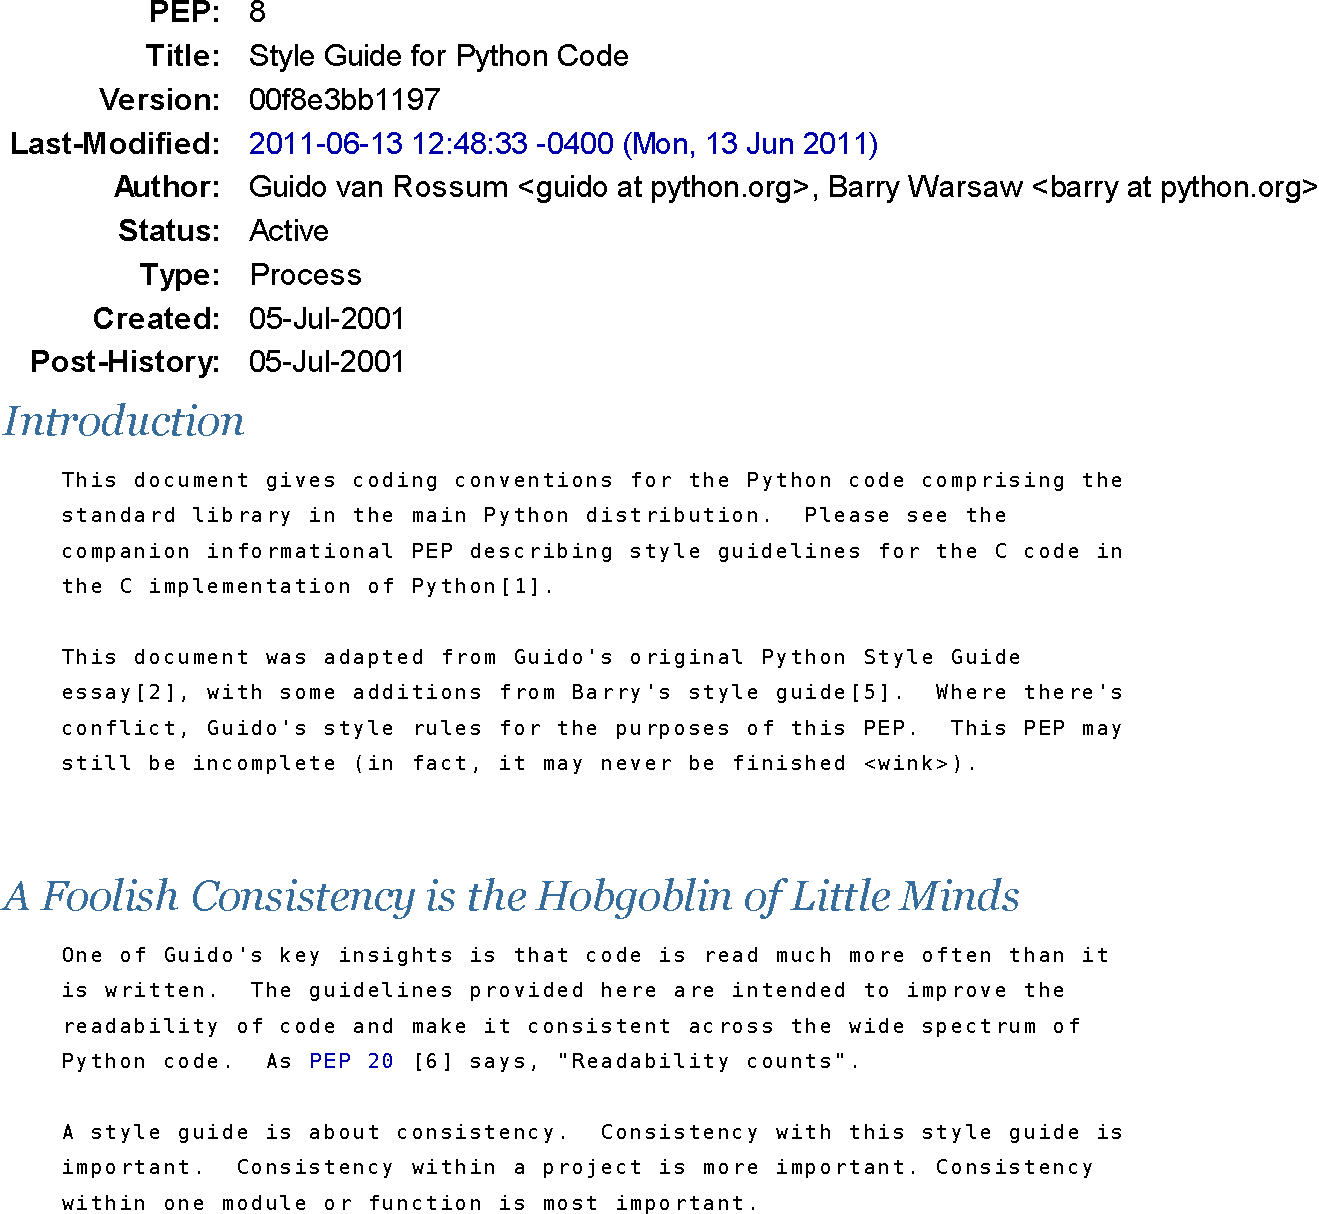
\includegraphics[width=\textwidth]{python/pep8}
  \caption{Excerpt from \ac{PEP} 8: Style Guide for Python Code.}
\end{figure}

The Python project defines three types of \acp{PEP}.

\begin{description}

  \item[Standards Track PEP] The most common form of \acp{PEP} describes a
    feature proposal for the Python language. They always consist of a design
    document and a reference implementation.

  \item[Informational PEP] Unlike the Standards Track \ac{PEP}, this type for
    \ac{PEP} does not propose a new feature. It provides general guidelines or
    information about a certain issue of Python. However it does not
    necessarily reach consensus inside the Python community and so one is free
    to ignore Informational \acp{PEP}.

  \item[Process PEP] This kind of \ac{PEP} is quite like the Standards Track
    \ac{PEP}, except that it applies to other areas than the Python language
    and describes processes around Python. For example any guidelines, decision
    making processes, development workflow and so on are mostly a Process
    \ac{PEP}. Additionally any \acp{PEP} which describe other \ac{PEP}, for
    example how a \ac{PEP} should look like, will be seen as a Process \ac{PEP}
    too.

\end{description}

The \ac{PEP} process begins with a feature proposal for Python. While all
bigger proposals require a \ac{PEP}, the Python project suggests to submit
small change directly as a patch submission. A \ac{PEP} always has one or
several authors, who have the responsibility for it. They will begin by
submitting the \ac{PEP} to the Python project. More precisely it should be
presented to the python-ideas mailing list and subsequently sent to the
\ac{PEP} editors. The \ac{PEP} editors will assign a number and a category as
mentioned above. Additionally, new \acp{PEP} always start with the \emph{Draft}
status. From there, the \ac{PEP} workflow begins.

\begin{figure}[htbp]
  \centering
  \begin{tikzpicture}[auto]
   \node[rectangle, rounded corners, draw=black, text width=6.5em, minimum height=2em, text centered]
     (draft) {Draft};
   \node[below=0.5cm of draft, rectangle, rounded corners, text width=6.5em, minimum height=2em, text centered]
     (dummy) {};
   \node[below=0.5cm of dummy, rectangle, rounded corners, draw=black, text width=6.5em, minimum height=2em, text centered]
     (deferred) {Deferred};

   \node[right=1cm of draft, rectangle, rounded corners, draw=black, text width=6.5em, minimum height=2em, text centered]
     (accepted) {Accepted};
   \node[below=0.5cm of accepted, rectangle, rounded corners, draw=black, text width=6.5em, minimum height=2em, text centered]
     (rejected) {Rejected};
   \node[below=0.5cm of rejected, rectangle, rounded corners, draw=black, text width=6.5em, minimum height=2em, text centered]
     (withdrawn) {Withdrawn};

   \node[right=1cm of accepted, rectangle, rounded corners, draw=black, text width=6.5em, minimum height=2em, text centered]
     (final) {Final};
   \node[below=0.5cm of final, rectangle, rounded corners, draw=black, text width=6.5em, minimum height=2em, text centered]
     (replaced) {Replaced};
   \node[below=0.5cm of replaced, rectangle, rounded corners, draw=black, text width=6.5em, minimum height=2em, text centered]
     (active) {Active};

   \draw[draw, -latex] ($(draft.south) - (1cm,0)$) -- ($(deferred.north) - (1cm,0)$);
   \draw[draw, -latex] ($(deferred.north) - (0.5cm,0)$) -- ($(draft.south) - (0.5cm,0)$);
   \path[draw, -latex] ($(draft.south) + (0.5cm,0)$) |- (rejected);
   \path[draw, -latex] (draft) |- ($(withdrawn.west) + (-0.5cm,0.8cm)$) |- (withdrawn.west);

   \draw[draw, -latex] (draft.east) -- (accepted.west);
   \draw[draw, -latex, dashed] (accepted.south) -- (rejected.north);

   \draw[draw, -latex] (accepted.east) -- (final.west);
   \draw[draw, -latex, dashed] (final.south) -- (replaced.north);
  \end{tikzpicture}
  \caption{Possible paths of the status of \aclp{PEP}.}
\end{figure}

\paragraph{Draft}

This is the default state of any new \ac{PEP} on submission, as described
above.

\paragraph{Deferred}

A \ac{PEP} Editor can always, instead of assigning the Draft status, defer a
\ac{PEP}. Reasons for a deferral could be duplication, being poorly written,
lack of motivation by the author or not being in line with the Python
philosophy.

\paragraph{Accepted}

A \ac{PEP} will be able to get this status assigned, if all \ac{PEP} criteria
are matched. This includes a precise formulation of the \ac{PEP}, not breaking
backwards compatibility and finally be accepted by the \ac{BDFL}. However the
criteria are not set in stone and basically a \ac{PEP} just have to be accepted
by the \ac{BDFL} to get accepted.

\paragraph{Rejected}

At this stage a \ac{PEP} can still be rejected. Mostly this status gets
assigned, if it turns out that the original idea did not fit the Python project
that well. But basically it is just a option to drop a \ac{PEP} even, after it
was either accepted or not deferred.

\paragraph{Withdrawn}

A \ac{PEP} can also always be withdrawn by the author of a \ac{PEP}. This could
help if an author does not want to work on a \ac{PEP} anymore, for example
because there is a better solution available.

\paragraph{Final}

Once a \ac{PEP} has been accepted and has a reference implementation available,
it can get the status Final by the \ac{BDFL}.

\paragraph{Replaced}

Mostly for Informational \acp{PEP}, subsequent versions can replace a \ac{PEP}.
In this case the original \ac{PEP} would be marked as Replaced and superseded
by the new \ac{PEP}.

\paragraph{Active}

Informational and Process \ac{PEP} can also be marked as Active, if they never
will be completed. For example \ac{PEP} 1 \cite{Warsaw2000}, which describes
the process of \acp{PEP} has it's status set to Active, as it is continually
improved and adapted to new workflows.

\begin{figure}[htbp]
  \centering
  \includegraphics[width=0.8\textwidth]{python/authors_by_month}
  \caption{Amount of distinct authors of CPython over time. Python~2 seemed to
  provide a major reason for developers to join.}
\end{figure}

% }}}

% }}}
